\chapter{Bayesian Inference}
\label{chap:bay}
%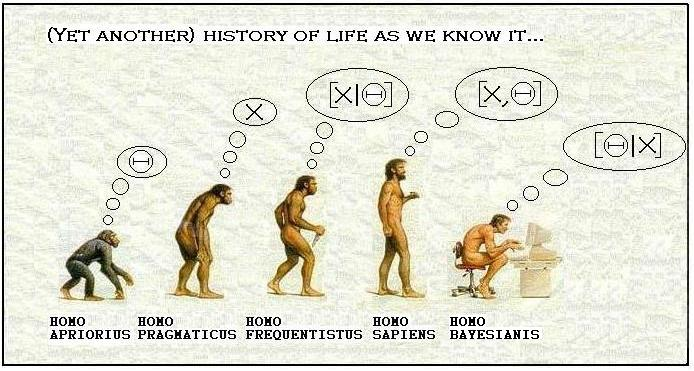
\includegraphics[width=\textwidth]{bayesian_evol}

\epigraph{We anticipate the sun will rise tomorrow, not just because it has always done so far, but because this is predicted by {\em models}, which accord with {\em data}. Any perceived failure of the sun to rise would more likely be a hallucination.}{\davidmackay{}}

%  * BRIEF intro to difference between bayesian and frequentist, and the nature of probability
%      - Continuous vs. Discrete
%      - Aleatoric vs. Epistemological \davidspiegelhalter
%
%  * Parameter estimation and model comparison
%       -Example? (e.g.\ coin flipping, --- anything better?)
%
%  * Sampling as method for describing high-dimensional probability distributions.
%      - MH as good technique
%      - Need for evidences


Science is not the search for truth. Instead, scientists concern themselves with the construction of models. These models have their relative merit determined using data.\footnote{The opening statement of this chapter was in fact the first thing \rafiblumenfeld{} said to us for our part IB Physics supervisions.}

% Mathematics -- if then, conditional truth
% Science -- weaker: observations -> possibilities 

\section{Probability}
\label{sec:bay:prob}

Probability is the mathematical language of uncertainty. It is a methodology of assigning a numerical weighting to outcomes or {\em events}. An event is any subset of the sample space $\Omega$. Some examples of discrete and continuous sample spaces are:
\begin{enumerate}
  \item The outcome of a coin flip $\Omega_1=\{\mathrm{Heads},\mathrm{Tails}\}$.
  \item The measured position of an electron $\Omega_2=\mathbb{R}$.
\end{enumerate}
For example, an event could be that the electrons position $x$ is measured to be $-1<x<0.5$. The role of probability is to assign a weighting to all subsets, which roughly corresponds to the ``chance'' that such an event would occur. Probability should therefore be additive:
\begin{equation}
  A,B \mathrm{\ disjoint} \Rightarrow \Prob{A \cup B} = \Prob{A} + \Prob{B}.
  \label{eqn:bay:add}
\end{equation}
One also normalises the probability distribution so that $\Prob{\Omega} = 1$. The above is effectively a paraphrasing of Kolmogorov's axioms of probability.

%In addition, if one has two disjoint sample spaces, for example $\Omega_1$ and $\Omega_2$ mentioned above, one may combine these into a single samples space ${\Omega=\Omega_1\otimes\Omega_2}$, then probability should be multiplicative.





This entire section may be summarised succinctly and formally as:
\begin{quote}
  Probability is any additive mapping $\mathrm{P}$ from the power set $2^\Omega$ of the sample space $\Omega$ to $[0,1]\in \mathbb{R}$, such that $\Prob{\Omega}=1$.
\end{quote}
\johnskilling{} has derived probability from measurement-theoretical grounds\citep[chap. 1]{Bayesian_methods_in_cosmology}, which provides a more intuitive backing to the definition.




\subsection{Bayes' theorem}


\begin{figure}
  \centerline{%
    \def\firstcircle{(-0.75,0) circle (1.5)}
\def\secondcircle{(0.75,0) circle (1.5)}

\begin{tikzpicture}
  \draw \firstcircle;
  \draw \secondcircle;
  \draw (-3,-2) rectangle (3,2);

  \begin{scope}
    \fill[blue!30!white] \firstcircle;
    \clip \secondcircle;
  \end{scope}

  \begin{scope}
    \clip \firstcircle;
    \fill[blue!60!white] \secondcircle;
  \end{scope}

  \draw[above left] node at (-1,0) {\(A\)};
  \draw[above right] node at (1,0) {\(B\)};
  \draw[below ] node at (0,0) {\(A\cap B\)};
  \draw[below left] node at (3,2) {\(\Omega\)};


\end{tikzpicture}


  }
  \caption{Beer-mat mathematics. This diagram is how \edjaynes{} explained Bayes' theorem to a young \stevegull{}. Out of the entire sample space $\Omega$, if we observe $A$ to be true (blue region), then the probability of $B$ given that we know $A$ is simply $\Prob{A\cap B}/\Prob{A}$. Bayes' theorem then follows by rearrangement and symmetry.}
\end{figure}


From this definition, it is useful to define conditional probability via:
\begin{equation}
  \Probc{B}{A} = \frac{\Prob{A\cap B}}{\Prob{A}}.
  \label{eqn:bay:cond}
\end{equation}
Multiplying both sides by $\Prob{A}$, and noting the symmetrical alternative:
\begin{equation}
  \Probc{B}{A}\Prob{A} = \Prob{A\cap B} = \Probc{A}{B}\Prob{B},
  \label{eqn:bay:sym}
\end{equation}
one may then derive Bayes' theorem:
\begin{align}
  \Probc{B}{A} &= \frac{\Probc{A}{B}\Prob{B}}{\Prob{A}}.\\
  \label{eqn:bay:bayes}
  \tag{Bayes' Theorem}
\end{align}
\section{Bayesian vs.\ Frequentist}
\label{sec:bay:bayesian_frequentist}

Whilst the previous section outlined the properties that probability must satisfy, it has not detailed how one should assign probability. Indeed, we have merely referred to probability as a measure of ``chance'', but declined to define what this means.

There are two fundamental types of probability: {\em Aleatoric\/} and {\em Epistemological}. Aleatoric systems are genuinely random, for example: the flip of a coin, or the click on a Geiger counter. Epistemological probability governs systems where the randomness is associated with a subjective lack of knowledge. For example, before prince George was born, bookmakers took bets on whether William and Kate's baby was a boy or a girl. 

The Frequentist school of thought defines probability as:
\begin{description}
  \item[Frequentist Probability:]``The limiting relative frequency of an event.''
\end{description}
I.e.\ if a coin has $\Prob{\mathrm{Head}}=\frac{1}{2}$, then if you were to toss it an arbitrarily large number of times, the fraction of times one would get closer and closer to $\frac{1}{2}$. This is the version of probability that most people encounter early in their mathematical education, but it has several issues.

This definition applies relatively well to Aleatoric systems (since an experiment can often be run a large number of times). However, for epistemological systems, it is all but useless. The frequentist solution is therefore to disregard the latter kind of probability.

Most people's experiences with probability will likely involve betting scenarios, such as William and Kate's baby. Here it is obvious that the betting odds should be approximately $1:1$,\footnote{Betting odds of $a:b$ against indicates a probability of success of $\frac{b}{a+b}$.}\footnote{In fact the probability of a boy being conceived across the population is roughly 51\%, in order to biologically account for male infant mortality. An individual's probability of conceiving a boy or a girl will vary from person to person and in time.}\footnote{A good bookmaker will obviously take this into account, and give you slightly worse odds in order to ensure their profit.} but it should be also be clear that these odds most certainly do not refer to an event that can be repeated an arbitrarily large number of times.

The alternative definition of probability is {\em Bayesian\/}:
\begin{description}
  \item[Bayesian Probability:] ``A degree of belief that an event will occur.'' 
\end{description}
Note that Bayesian probability is {\em subjective}, it matters who's degree of belief one is considering. Probabilities are assigned only with a given state of knowledge. Effectively, Bayesians place aleatoric and epistemological probability under the same umbrella. 

Pure mathematics deals in relative truth or falsity, i.e.\ given initial assumptions, all statements are assigned to the set $\{F,T\}\equiv\{0,1\}$. Bayesian probability can be thought of as a blurring of this process, namely from initial assumptions, various conclusions are assigned a number from the continuum between $[0,1]$.

\section{An example: biased coins}
For example, assume that you toss a coin $N=20$ times, and observe a dataset of $\data = 16$ heads. Is this enough to cause us to doubt the fairness of the coin?

The standard model $\model_0$ is that a coin toss consists of a binomial trial with probability $\frac{1}{2}$. Elementary probability tells us that the chance of getting this data is:
\begin{equation}
  \Probc{\data}{\model_0}= {^{N}C_\data} {\left( \frac{1}{2} \right)}^{N}  = 4.6\times 10^{-3}.
  \label{eqn:bay:M0}
\end{equation}
Note that as should be expected, the chance of obtaining this exact dataset is small. 

If we allow for the possibility that the coin could be any probability $p$, we can encapsulate this in a second model $\model_1$.
\begin{equation}
  \Probc{\data}{p,\model_1}= {^{N}C_\data}\: {p}^{\data} {\left(1 - p \right)}^{N-\data} 
  \label{eqn:bay:M1}
\end{equation}
This second model is not ideal, since we haven't specified the parameter $p$. If we choose $p=\frac{1}{2}$ we recover $\model_0$. It is tempting to choose $p$ such that the probability of getting the data is maximised. This would be an example of a {\em maximum likelihood\/} approach. In this case, the method indicates\footnote{Proof left as exercise to the reader.} we should choose $p = \frac{\data}{N}$. 

Maximum likelihood has its drawbacks, particularly in the case of a low volume of data. After $N=1$ toss, it seems a little premature to choose either $p=1$ or $p=0$ depending on whether we see a head or a tail. Instead picking a specific value of $p$, one could instead ``spread your bets'' and consider several different values of $p$. The full generalisation of this is to consider a continuum of models, and define an initial probability distribution $\Probc{p}{\model_1}$. These can be interpreted as our initial assumptions on the value of $p$, or our initial degree of belief in its value
A natural assumption is to try and be as unbiased as possible and assume that $p$ is equally likely to take any value in between $0$ and $1$. We therefore have:
\begin{equation}
  \Probc{p}{\model_1}=\left\{
  \begin{array}{lr}
    1 &:0\le p\le1\\
    0 &:\text{otherwise.}\\
  \end{array}
  \right.\label{eqn:bay:prior1}
\end{equation}
With this distribution, we can work out what the overall probability of obtaining the dataset $\data$ is, by marginalising over all values of $p$:
\begin{align}
  \Probc{\data}{\model_1} 
  &= \int \Probc{\data}{p,\model_1}\Probc{p}{\model_1}\: dp \\
  &= \int_0^1 {^{N}C_\data}\: {p}^{\data} {\left(1 - p \right)}^{N-\data}\: dp \\
  &= \frac{1}{n+1} = 4.8\times10^{-2}
  \label{eqn:bay:marg}
\end{align}
This is quite telling, because our initial choice for $\Probc{p}{\model_1}$~(\ref{eqn:bay:prior1}) indicates that we expect all data sets with equal probability (independent of $\data$). This is therefore a ``minimally suspicious'' choice in spread.

We now have two equations~(\ref{eqn:bay:M0})~\&~(\ref{eqn:bay:marg}) which detail the probability of getting the dataset $\data$ given the choice of model. However, what we are really after is the probability of the model, given the dataset $\Probc{\model}{\data}$. To compute this, we use Bayes' theorem
\begin{equation}
  \Probc{\model}{\data} = \frac{\Probc{\data}{\model}\Prob{\model}}{\Prob{\data}}.
  \label{eqn:bay:bay_md}
\end{equation}
In order to complete the calculation, we must assign a probability to each model. A natural choice is to consider $\Prob{\model_0}=\Prob{\model_1}=\frac{1}{2}$. $\Prob{\data}$ is just a normalising constant, computed as:
\begin{equation}
  \Prob{\data} = \sum_i \Probc{\data}{\model_i}\Prob{\model_i}, 
  \label{eqn:bay:norm}
\end{equation}
so we may finally compute
\begin{equation}
  \Probc{\model_0}{\data} = 0.088 \qquad
  \Probc{\model_1}{\data} = 0.922
  \label{eqn:bay:comp}
\end{equation}
In other words, a betting man would put money on $\model_1$ with odds of $10:1$ for. Another way of thinking of this is that $\model_1$ is ten times better at describing the data than $\model_0$.

$\model_1$ can go further however. We may also use Bayes' theorem to compute 
\begin{equation}
  \Probc{p}{\data,\model_1} = \frac{\Probc{\data}{p,\model_1}\Probc{p}{\model_1}}{\Probc{\data}{\model_1}}.
  \label{eqn:bay:bay_p}
\end{equation}
This here gives us the distribution on $p$ {\em given the data}. Namely, how the data should update our ``spread bet''. We already have the ingredients for the above construction from equations~(\ref{eqn:bay:M1}),~(\ref{eqn:bay:prior1}),~\&~(\ref{eqn:bay:marg}), and given the uniform prior, we find our updated bet on $p$ is proportional to $p^\data{(1-p)}^{N-\data}$, a function of $p$. This is a beta distribution, and is indicated in Figure~\ref{fig:bay:beta}.

\begin{figure}
  \centerline{%
    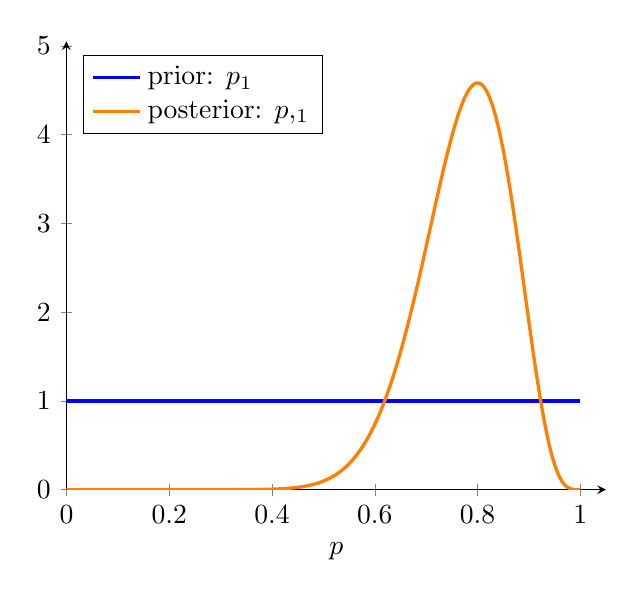
\begin{tikzpicture}[
    declare function={%
      beta(\p,\d,\n)=\p^\d * (1-\p)^(\n-\d) /factorial(\d)/factorial(\n-\d)*factorial(\n+1);
    }
  ]

  \begin{axis}[
      axis lines=left,           % Don't draw box axes
      ymax=5.05,                    % to ensure number 5 is included
      samples=100,               % any fewer and it looks weird
      domain=0:1,                % x range
      xlabel=$p$,                % x label
      xmax=1.05,
      legend cell align=left,    % align legend text left
      legend pos= north west,    % put legend in top left
    ]

    \def\pdata{16}    % Number of heads
    \def\pnumber{20}  % Number of coin flips

    % Draw the prior
    \addplot [very thick,blue] {1}; 
    % Add the prior legend
    \addlegendentry{prior: $\Probc{p}{\model_1}$}

    % Draw the posterior
    \addplot [samples=200,very thick,orange] {beta(x,\pdata,\pnumber)}; 
    % Add the posterior legend
    \addlegendentry{posterior: $\Probc{p}{\data,\model_1}$}

  \end{axis}
\end{tikzpicture}

  }
  \caption{%
  Beta function.\label{fig:bay:beta}
}
\end{figure}

\section{Parameter Estimation \& Model Comparison}
\label{sec:bay:model_comp}
We shall now take the concepts of the previous section, and put them in a general setting. 

The typical problem of science is the construction of a model $\model$ in order to explain some dataset $\data$. Typically, scientific models have a set of continuous parameters $\params_\model$, where $\params_\model$ is normally multi-dimensional, and may contain a variety of parameter types such as integers, vectors, tensors and more exotic components.

Elementary probability theory then enables us to calculate the probability of the data, given the choice of model along with a specific parameter choice.
\begin{equation}
  \lik\equiv\Probc{\data}{\params_\model,\model}.
  \label{eqn:bay:lik_def}
\end{equation}
This distribution is called the {\em likelihood}, which is denoted with a calligraphic~$\lik$ to differentiate between rapidly proliferating conditional probabilities. It is also clearer in many situations to supress explicit data, model and/or parameter-dependence of the likelihood, and instead write:
\begin{equation}
  \Probc{\data}{\params_\model,\model}
  \equiv
  \lik_\model(\params_\model)
  \equiv
  \lik(\params)
  \equiv
  \lik_\model
  \equiv
  \lik.\nonumber
\end{equation}
This is a generic overloading technique which I utilise throughout this thesis.

In order to perform Bayesian inference, another requirement of the model $\model$ is that it must specify an initial degree of knowledge of the parameters:
\begin{equation}
  \prior\equiv\Probc{\params_\model}{\model}.
  \label{eqn:bay:prior_def}
\end{equation}
Since no model occurs in isolation, it is generally not difficult to theoretically produce upper and lower bounds on parameter values. The normal strategy is to choose fairly conservative uniform or Gaussian priors on parameter values. In general, the prior should encapsulate the scale and spread of our current expectation of the parameter value.

Once a prior has been specified, the model $\model$ is complete. The scientific aspect of the problem is complete, and the rest mere statistics. Statistical analysis may be neatly partitioned into two problems: {\em model comparison\/} and {\em parameter estimation}.

\subsection{Model comparison}
It is usually the case in science that there is not a single model available to explain the data. Typically one will have a set of models ${\{\model_1,\model_2,\ldots\}}$, which we wish to scientifically determine the relative merits of given the data $\data$.

We may use the prior to marginalise out all parameter dependence of the each model:
\begin{equation}
  \ev\equiv\Probc{\data}{\model} 
  =
  \int  \Probc{\data}{\params_\model,\model}\Probc{\params_\model}{\model}\:d\params_\model.
  \label{eqn:bay:ev_def}
\end{equation}
This quantity is termed the {\em evidence\/} $\ev$, or {\em marginalised likelihood}, and gives the probability of observing the data $\data$, conditioned on the model $\model$. The quantity we seek however is the probability of each model $\model$ given the data $\data$, which may be obtained using Bayes' theorem:
\begin{equation}
  \Probc{\model_i}{\data} = \frac{\Probc{\data}{\model_i}\Prob{\model_i}}{\Prob{\data}}.
  \label{eqn:bay:bayM}
\end{equation}
In order to utilise this however, we must specify our prior degree of belief in each model
\begin{equation}
  \Prob{\model_i} = \priorM_i
\end{equation}
These may have been obtained from previous analyses, but a non-partisan choice would be too choose the models to be equally weighted. The denominator of~(\ref{eqn:bay:bayM}) is then simply a normalising constant, and the posterior degree of belief in each model may be obtained via:
\begin{equation}
  \Probc{\model_i}{\data} 
  \equiv
  \Wmodel_i
  =
  \frac{\ev_i\priorM_i}{\sum_j \ev_j\priorM_j}.
\end{equation}
These model weights $\Wmodel$ may then be used to determine the ``most probable model''. In some cases there is a clear winner, and the other models may be safely discarded, but the more usual scenario is that there are several competing alternatives. It is for this reason that we prefer the term ``model comparison'' to the more oft-quoted {\em model selection}. Additional datasets may determine a clear winner, but in the mean-time the weights $\Wmodel$ can be used to perform proper inference. 

For example, model often predict a distribution for a common derived parameter $\Probc{y}{\model,\data}$.\footnote{E.g.\ in cosmology, various models of the universe will predict an age or curvature of the cosmos} If the data are not strong enough to distinguish a given model, the correct inference on $y$ is to use a posterior which marginalises over all models:
\begin{equation}
  \Probc{y}{\data} 
  = \sum_i\Probc{y}{\data,\model_i}\Probc{\model_i}{\data}
  = \sum_i\Probc{y}{\data,\model_i}\Wmodel_i.
\end{equation}
This fully Bayesian approach has been historically under-utilised due to the difficulties in numerically computing the evidence.



\subsection{Parameter estimation}
Of equal interest to scientists is to ask what the data tells us about the various parameters.  
Bayes' theorem allows us to invert the conditioning in equation~(\ref{eqn:bay:lik_def}) and find the {\em posterior\/} $\posterior$ by combining the likelihood~(\ref{eqn:bay:lik_def}), prior~(\ref{eqn:bay:prior_def}) and evidence~(\ref{eqn:bay:ev_def}):
%
\begin{equation}
  \posterior\equiv
  \Probc{\params_\model}{\data,\model} = \frac{\Probc{\data}{\params_\model,\model} \Probc{\params_\model}{\model}}{\Probc{\data}{\model}},
  \label{eqn:bay:bayes_theorem}
\end{equation}
%
which is schematically written as:
\begin{align}
  \posterior &= \frac{\lik \times \prior }{\ev }
  \label{eqn:bay:bayes_theorem_abbrv}\\
  \mathrm{Posterior} &= \frac{\mathrm{Likelihood} \times \mathrm{Prior} }{\mathrm{Evidence} }
\end{align}
This describes how our initial knowledge $\prior$ of the parameters updates to $\posterior$ in light of the data $\data$. Note that the evidence $\ev$ features in both model selection and parameter estimation, and its computation is therefore of great significance.







\section{Numerical statistics: Sampling}
\label{sec:bay:samp}
Having discussed the theory of Bayesian statistics, we now turn to the more tricky aspect of actually computing these various inferences. The likelihood~(\ref{eqn:bay:lik_def}) $\lik(\params)$ is a routine, if often challenging, quantity to compute. It is the job of observational scientists to provide this function, and for the purposes of inference we may consider it a ``black box''. In general, $\lik$ will be not be analytical, but instead is a numerical and computationally expensive quantity. Any calculation we perform must aim to minimise the number of times we attempt to evaluate $\lik$. The prior $\prior$ is typically much less expensive to compute and is normally expressed using analytic functions such as a uniform or Gaussian distribution.

Typically, in inference calculation we wish to compute quantities that are marginalised over by the posterior. For example means and variances will typically take the form:
\begin{align}
  \mean{f} 
  &= \int f(\params)\posterior(\params)\:d\params,
  \label{eqn:bay:mean}\\
  &= \int f(\params)\frac{\lik(\params)\prior(\params)}{\ev}\:d\params.
\end{align}
Given a likelihood $\lik$ and a prior $\prior$, a naive approach would be to first compute the evidence
\begin{equation}
  \ev = \int \lik(\params) \prior(\params) \: d\params,
  \label{eqn:bay:ev_short}
\end{equation}
and then perform the integral~(\ref{eqn:bay:mean}) using a traditional numerical quadrature procedure. In most cases, this method fails at both steps, due to the fact that the dimensionality of the integration is too high for numerical quadrature to succeed.

To see this issue, consider the integration of a function $g$ along $[0,1]$
\begin{equation}
  \int_0^1 g(x) dx \approx \sum\limits_{i=0}^{n} g(x_i) w_i,
\end{equation}
where ${x_i\in[0,1]}$ are the quadrature points ${w_i\in\mathbb{R}}$ are the quadrature weights. For example, if $x_i = \frac{i}{n}$ and $w_i=\frac{1}{n+1}$ then one obtains the left rectangle rule (Figure~\ref{fig:bay:quadrature}). This calculation therefore requires $\bigO{n}$ calculations of the function In the $d$-dimensional case, then one has the generalisation:
\begin{equation}
  \int_0^1\cdots\int_0^1 g(x_1,\cdots,x_d) dx_1\cdots \: dx_d \approx \sum\limits_{i_1,\cdots,i_d=0}^{n} g(x_{i_1},\cdots,x_{i_d}) w_{i_1,\cdots,i_d},
\end{equation}
This calculation however requires $\bigO{n^d}$ function evaluations. This is an exponential scaling with $d$, and is an example of the {\em curse of dimensionality}. Even for modest number of parameters $\left[ d\bigO{4} \right]$ these kind of integrations require unfeasible amounts of computational time. Worse still, for most likelihoods, the region about which $\lik$ is significantly non-zero is much larger than the prior range\footnote{This should be expected, since the data should update the prior by some amount in each dimension.}. The gridding size $n$ must therefore be taken as reasonably large in order to ensure that enough function evaluations occur at the peak.

\begin{figure}
  \centerline{%
    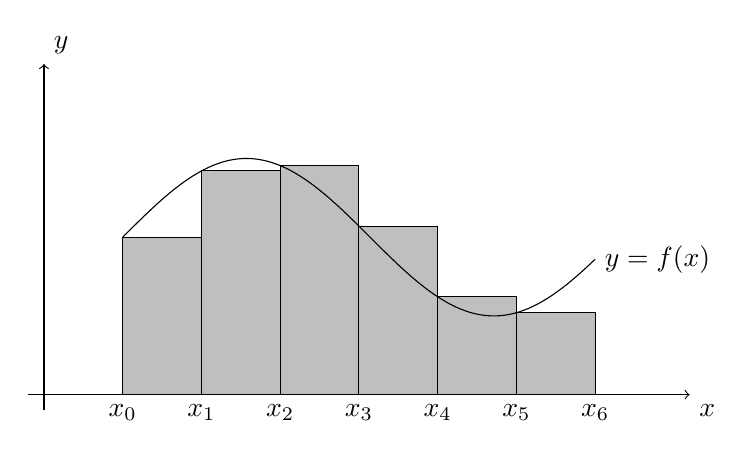
\begin{tikzpicture}
  \draw[->] (-.2,0) -- (8.2,0) node[below right] {$x$};
  \draw[->] (0,-.2) -- (0,4.2) node[above right] {$y$};

  \foreach \x in {0,1,...,5} {%
    \draw[fill=gray!50] (\x + 1,0) -- ++(1,0) -- ++(0,{sin(\x r) ++ 2}) --
    ++(-1,0) -- ++(0,{-sin(\x r) - 2});
  }

  \draw[domain=0:6,samples=100] plot(\x + 1,{sin(\x r) + 2})
  node[right] {$y = f(x)$};

  \foreach \x in {0,1,...,6} {%
    \draw (\x + 1,0) node[below] {$x_{\x}$};
  }
\end{tikzpicture}

    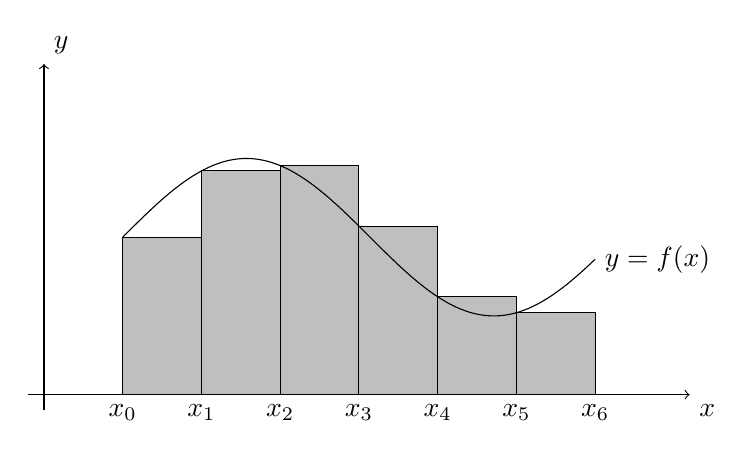
\begin{tikzpicture}
  \draw[->] (-.2,0) -- (8.2,0) node[below right] {$x$};
  \draw[->] (0,-.2) -- (0,4.2) node[above right] {$y$};

  \foreach \x in {0,1,...,5} {%
    \draw[fill=gray!50] (\x + 1,0) -- ++(1,0) -- ++(0,{sin(\x r) ++ 2}) --
    ++(-1,0) -- ++(0,{-sin(\x r) - 2});
  }

  \draw[domain=0:6,samples=100] plot(\x + 1,{sin(\x r) + 2})
  node[right] {$y = f(x)$};

  \foreach \x in {0,1,...,6} {%
    \draw (\x + 1,0) node[below] {$x_{\x}$};
  }
\end{tikzpicture}

  }
  \caption{\label{fig:bay:quadrature}}
\end{figure}

Fortunately there is a better way. Since we only need points within the region 




\section{Nested Sampling}




%Calculation of the posterior $\posterior(\theta)$ is the domain of {\em parameter estimation}, and in high dimensions is best performed by sampling the space with a Markov-Chain Monte-Carlo approach (MCMC). Examples include Metropolis-Hastings, Gibbs sampling and Slice sampling. For the most part, the evidence $\ev$ is ignored during such calculations, and one works with an unnormalised posterior ${\posterior\propto\lik\times\prior}$.




